\ifdefined\standalone
\documentclass[12pt]{article}
\usepackage{graphicx}
\usepackage{float}
\usepackage[a4paper, margin=1in]{geometry}
\usepackage[utf8]{inputenc}
\usepackage{textcomp}  % <-- for \textdegree
\usepackage{amsmath}
\usepackage[hidelinks]{hyperref} % <- hypertext
\usepackage{tikz}
\usetikzlibrary{decorations.pathmorphing,patterns}
\begin{document}
\fi

\section{Heat Conduction With Temperature-Dependent Thermal Properties}

A one-dimensional heat conduction problem through a planar slab of thickness $L = 1~\mathrm{cm}$ is considered.
The material is initially at a uniform temperature of $T_{\mathrm{ini}} = 0~^\circ\mathrm{C}$.
The front surface is exposed to a hot gas at $700~^\circ\mathrm{C}$, while the back surface is exposed to a gas at $0~^\circ\mathrm{C}$.
Heat transfer at both boundaries is governed exclusively by convection, with a constant convective heat transfer coefficient of $h_c = 10~\mathrm{W\cdot m^{-2}\cdot K^{-1}}$ (see Fig.\ref{fig:heat_conduction_kc_configuration}).
The thermal conductivity $k$ and the specific heat capacity $c_p$ are temperature-dependent. Their temperature evolution is assumed to be linear, and their values at some specific temperatures are reported in Table~\ref{tab:thermal_properties}. Note that Gpyro models temperature-dependent properties in the form $\phi(T) = \phi_0 \left(\frac{T}{T_\mathrm{ref}}\right)^n$, therefore, distinct coefficients $\phi_0$ and exponents $n$ are selected such that the resulting variation is locally quasi-linear and consistent with the reference data.

The results are presented in Fig.~\ref{fig:heat_conduction_kc_results}, where the numerical results are compared with those obtained using the finite-difference solver HEATING \cite{FDS_Verif,HEATING7}.

\begin{table}[H]
\centering
\caption{Thermophysical properties of the slab material.}
\label{tab:thermal_properties}
\renewcommand{\arraystretch}{1.3}
\begin{tabular}{c c c c}
\hline
Temperature ($^\circ\mathrm{C}$) &
$k$ ($\mathrm{W\,m^{-1}\,K^{-1}}$) &
$c_p$ ($\mathrm{J\,kg^{-1}\,K^{-1}}$) &
$\rho$ ($\mathrm{kg\,m^{-3}}$) \\
\hline
0   & 0.10 & 1000 & 10\,000 \\
100 & 0.15 & 1200 & 10\,000 \\
200 & 0.20 & 1000 & 10\,000 \\
\hline
\end{tabular}
\end{table}


\begin{figure}[htbp]
\centering

\begin{minipage}{0.48\textwidth}
\centering
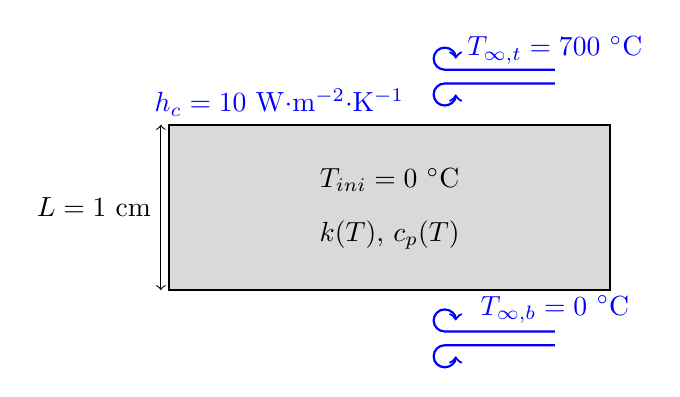
\begin{tikzpicture}[scale=0.7]

\draw[fill=gray!30,thick] (0,0) rectangle (8,3);
\node at (4,2) {$T_{ini} = 0~^\circ\mathrm{C}$};
\node at (4,1) {$k(T)$, $c_p(T)$};

\draw[<->] (-0.15,0) -- (-0.15,3);
\node[left] at (-0.15,1.5) {$L = 1$~cm};

% Convective arrows
\draw[->,thick, blue] (7,3.75) -- (5,3.75) arc[start angle=90, end angle=360, radius=0.2cm];
\draw[->,thick, blue] (7,4) -- (5,4) arc[start angle=270, end angle=0, radius=0.2cm];

\node[blue] at (2,3.4) {$h_c = 10~\mathrm{W{\cdot}m^{-2}{\cdot}K^{-1}}$};
\node[blue] at (7,4.35) {$T_{\infty,t} = 700~^\circ\mathrm{C}$};

\draw[->,thick, blue] (7,-1) -- (5,-1) arc[start angle=90, end angle=360, radius=0.2cm];
\draw[->,thick, blue] (7,-0.75) -- (5,-0.75) arc[start angle=270, end angle=0, radius=0.2cm];

\node[blue] at (7,-0.35) {$T_{\infty,b} = 0~^\circ\mathrm{C}$};

\end{tikzpicture}
\caption{Configuration schematic}
\label{fig:heat_conduction_kc_configuration}
\end{minipage}
\hfill
\begin{minipage}{0.48\textwidth}
\centering
\includegraphics[width=\textwidth]{heat_conduction_kc_results.png}
\caption{Evolution of front and back temperatures with time}
\label{fig:heat_conduction_kc_results}
\end{minipage}

\end{figure}



\ifdefined\standalone
\bibliographystyle{unsrt}
\bibliography{heat_conduction_kc}
\end{document}
\fi
